

\tikzset{every picture/.style={line width=0.75pt}} %set default line width to 0.75pt        

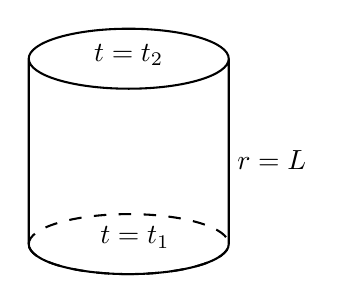
\begin{tikzpicture}[x=0.75pt,y=0.75pt,yscale=-1,xscale=1]
	%uncomment if require: \path (0,133); %set diagram left start at 0, and has height of 133
	
	%Shape: Ellipse [id:dp6649407092526456] 
	\draw  [dash pattern={on 4.5pt off 4.5pt}] (264,110.78) .. controls (264,102.79) and (285.57,96.32) .. (312.18,96.32) .. controls (338.79,96.32) and (360.37,102.79) .. (360.37,110.78) .. controls (360.37,118.76) and (338.79,125.23) .. (312.18,125.23) .. controls (285.57,125.23) and (264,118.76) .. (264,110.78) -- cycle ;
	%Shape: Can [id:dp9560851582958649] 
	\draw   (360.37,21.45) -- (360.37,110.78) .. controls (360.37,118.76) and (338.79,125.23) .. (312.18,125.23) .. controls (285.57,125.23) and (264,118.76) .. (264,110.78) -- (264,21.45) .. controls (264,13.47) and (285.57,7) .. (312.18,7) .. controls (338.79,7) and (360.37,13.47) .. (360.37,21.45) .. controls (360.37,29.44) and (338.79,35.91) .. (312.18,35.91) .. controls (285.57,35.91) and (264,29.44) .. (264,21.45) ;
	
	% Text Node
	\draw (363,64) node [anchor=north west][inner sep=0.75pt]    {$r=L$};
	% Text Node
	\draw (294,13) node [anchor=north west][inner sep=0.75pt]    {$t=t_{2}$};
	% Text Node
	\draw (297,101) node [anchor=north west][inner sep=0.75pt]    {$t=t_{1}$};
	
	
\end{tikzpicture}